\documentclass[nobib]{MSword}

% Preamble code:
%%%%%%%%%%%%%%%%%%%%%%%%%%%%%%%%%%%%%%%%
\usepackage[english]{babel}
\usepackage{csquotes}
\usepackage{lipsum}
\usepackage{graphicx}
\setlength{\parindent}{20pt}
\graphicspath{ {./images/} }

\title{PS6}
\author{Becky Crouse}
\date{March 21, 2023}

\begin{document}

\maketitle

\subsection*{Data Cleaning}
I'm utilizing ISORA data for this project. ISORA, or International Survey on Revenue Administration, is an international survey of revenue agencies which gathers metrics on taxpayer audits, assessments, and agency staffing. I utilize three data sets (5, 7, and 10) found online here: \url{https://data.rafit.org/?sk=8b008788-ebde-4d61-bc90-7438d6aa12dc&sId=1637191076670}. 

Because each of these files is formatted slightly differently, I read in and clean each file separately by performing the following steps:
\begin{enumerate}
  \item Read in the data and subset it to remove upper rows and extra columns that I'm not using.
  \item Adjust the column headings to reflect the first row headings.
  \item Repeat above for each data set. Because two of the files have two sets of information that I want, I end up with 5 data frames.
  \item I then convert each of the "wide" data frames to "long" data.
  \item I use SQLite in R to merge each of the "long" data frames together into a master data frame.
  \item I create new variables using the combined data.
  \item Finally, I do my final review and cleaning of the data. I remove any observations that are not readily interpreted: 
  \begin{itemize}
      \item Rows with missing information
      \item Countries reporting 0 taxpayers
      \item Countries reporting more audits than active taxpayers (audit rate >1)
  \end{itemize}
\end{enumerate}

\subsection*{Data Visualizations}
My interest in this data is in understanding how tax authorities differ on their audit aggressiveness as well as the taxpayers response. I created three visualizations to help me understand these relationships. 

First, I created scatter plots to visualize the data. I plot the audit rate (calculated as number of audits over the number of active taxpayers) against the total government revenue as a percent of GDP.

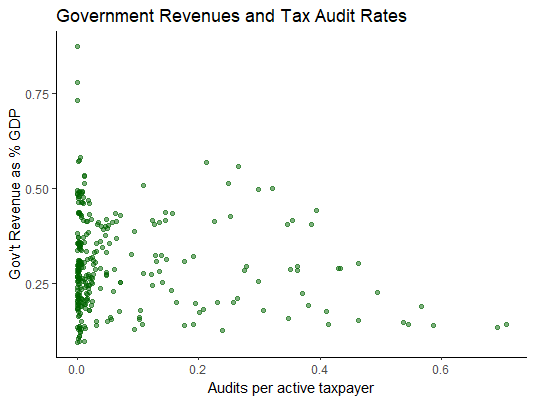
\includegraphics{images/PS6a_Crouse.png}

I then created a similar scatter plot, this time showing the rate of audits with assessment (calculated as number of audits with assessment over the number of active taxpayers) against the total government revenue as a percent of GDP.

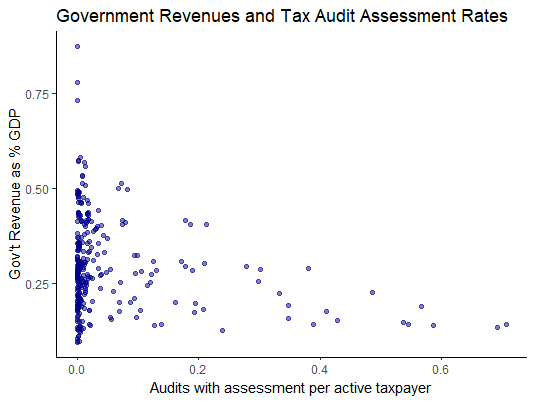
\includegraphics{images/PS6b_Crouse.png}

Finally, to understand the relationship between audit assessments and government revenue, I plotted a Loess curve of the regression of government revenue as a percent of GDP on audits with assessment. As expected, I find a significant negative relationship between these two, suggesting that audit assessments increase as government revenue falls (or vice versa). In untabulated analysis, I find a similar, though less significant, relationship between the overall audit rate and government revenues.

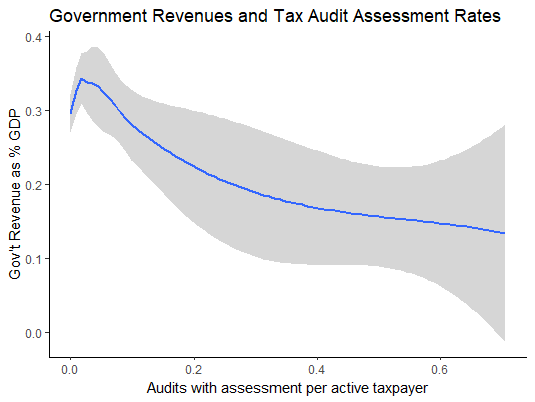
\includegraphics{images/PS6c_Crouse.png}

\end{document}